\documentclass[aspectratio=169]{beamer}
\usepackage[utf8]{inputenc}
\usetheme{SimpleDarkBlue}
\usecolortheme{default}
\usepackage{xcolor}
\usepackage{tikz}
\usepackage{hyperref}
\definecolor{IBMBlue}{RGB}{0,113,197}
\setbeamercolor{title}{bg=IBMBlue,fg=white}
\setbeamercolor{frametitle}{bg=IBMBlue,fg=white}
\title[DevOps i administrowanie]{Wprowadzenie do DevOps i zarządzania systemami}
\author{mgr inż. Jakub Woźniak}
\institute{Instytut Informatyki, Wydział Informatyki i Telekomunikacji Politechniki Poznańskiej}
\date{}

\begin{document}

\begin{frame}
\titlepage
\end{frame}

\begin{frame}{Agenda wykładu}
\tableofcontents
\end{frame}

\section{O przedmiocie}
\begin{frame}{O mnie}
\begin{itemize}
  \item \textbf{Jakub Woźniak} -- CTO, Software Services w Nordcloud, an IBM Company
  \item Specjalizacja: chmura publiczna i hybrydowa, developer experience, architektura oprogramowania
  \item Kontakt: \href{mailto:jakub.wozniak@cs.put.poznan.pl}{jakub.wozniak@cs.put.poznan.pl}\\\url{https://www.cs.put.poznan.pl/jwozniak}
\end{itemize}

\end{frame}

\begin{frame}{Cele przedmiotu}
\begin{block}{Cel główny}
Poznasz najnowocześniejsze praktyki zarządzania systemami rozproszonymi — DevOps, konteneryzacja, zadania współczesnego administratora / inżyniera DevOps.
\end{block}

\begin{itemize}
    \item Fundamenty DevOps
    \item Konteneryzacja i orkiestracja
    \item Automatyzacja infrastruktury (IaC)
    \item Monitorowanie i obserwability
    \item Strategie backup i recovery
    \item Wyzwania bezpieczeństwa w architekturach rozproszonych
\end{itemize}
\end{frame}

\section{Ewolucja roli administratora}
\begin{frame}{Ewolucja roli administratora}
\begin{itemize}
  \item 1990-2000: tradycyjny sysadmin, fizyczna infrastruktura, manualne wdrażanie
  \item 2000-2010: era wirtualizacji, centralizacja, powolna automatyzacja
  \item 2010-2025: „cloud-first”, Infrastructure as Code, DevOps, automatyzacja, SRE
\end{itemize}
\begin{center}
  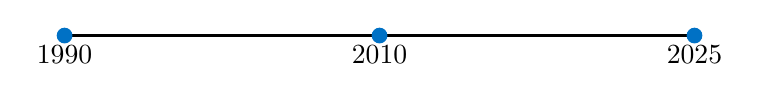
\begin{tikzpicture}
    \draw[thick] (0,0) -- (8,0);
    \fill[IBMBlue] (0,0) circle (0.1);
    \fill[IBMBlue] (4,0) circle (0.1);
    \fill[IBMBlue] (8,0) circle (0.1);
    \node[below] at (0,0) {1990};
    \node[below] at (4,0) {2010};
    \node[below] at (8,0) {2025};
  \end{tikzpicture}
\end{center}
\end{frame}

\section{Podstawy filozofii DevOps}
\begin{frame}{DevOps: definicja i geneza}
\begin{alertblock}{Definicja}
DevOps = Development + Operations, wspólna odpowiedzialność za cykl życia systemu IT
\end{alertblock}
\begin{itemize}
  \item „You Build It, You Run It” (Amazon)
  \item Szybsze wdrożenia, większa niezawodność, lepsza współpraca zespołów
  \item Historia: Patrick Debois, DevOpsDays 2009, rozwój praktyk SRE w Google
\end{itemize}
\end{frame}

\begin{frame}{Framework CALMS}
DevOps to nie tylko narzędzia, ale kultura i procesy.
\begin{description}
    \item[C] Culture (Kultura) -- współpraca, zaufanie, edukacja
    \item[A] Automation (Automatyzacja) -- CI/CD, IaC, automatyczne testy
    \item[L] Lean (Szczupłość) -- eliminowanie waste, małe zmiany, szybka informacja zwrotna
    \item[M] Measurement (Pomiary) -- metryki techniczne i biznesowe, monitorowanie, decyzje na podstawie danych
    \item[S] Sharing (Dzielenie się) -- dzielenie się wiedzą, otwarta komunikacja, cross-functionality
\end{description}
\end{frame}

\section{Współczesne trendy IT 2025}
\begin{frame}{Trendy 2025: AI, platformy, edge, green IT}
\begin{itemize}
    \item AI/ML w IT Operations (AIOps, detekcja anomalii, predykcja awarii)
    \item Platform Engineering – developer self-service, golden paths, Netflix Backstage
    \item Edge Computing – rozproszona infrastruktura, niskie opóźnienia dla IoT
    \item Sustainability – optymalizacja kosztów i emisji, cloud regions green
    \item Zero Trust – bezpieczeństwo oparte na tożsamości
\end{itemize}
\end{frame}

\section{Przykład: Transformacja DevOps w Santander Bank Polska}
\begin{frame}{Case study: Santander Bank Polska}
\textbf{Wyzwanie:} ręczne procesy, długie wdrożenia, złożoność compliance.\\
\textbf{Transformacja:} Jira, CI/CD, automatyzacja deploymentów, regulatory compliance zautomatyzowane.\\
\textbf{Efekty:} 70\% szybsze wdrożenia, większa stabilność, lepsza współpraca i audytowalność.
\end{frame}

\section{Podsumowanie}
\begin{frame}{Podsumowanie i zalecenia}
\begin{itemize}
    \item Administrator XXI wieku: inżynier systemowy, automatyk, partner dla biznesu
    \item DevOps: przede wszystkim zmiana kultury, potem narzędzia
    \item Kariery: Platform Engineering, DevSecOps, SRE, Cloud Native
\end{itemize}

\end{frame}

\end{document}
